\section{Présentation de la cellule automatisée}
\subsection{Matériel}

\begin{figure}[ht]
    \centering
    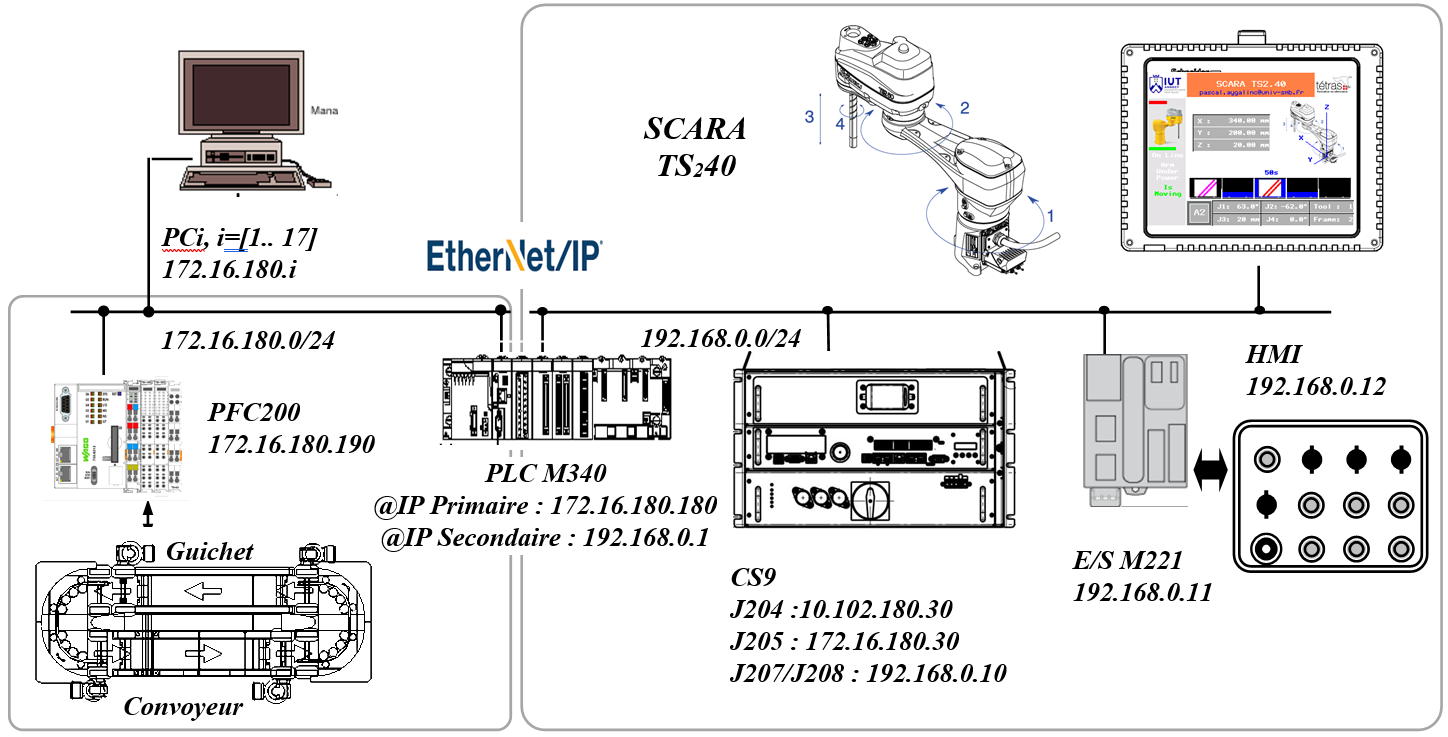
\includegraphics[width=0.8\linewidth]{architecture.png}
    \caption{Cellule robotisée}
    \label{fig:cellule}
\end{figure}


Pour réaliser ce TP, la cellule robotisée, représentée en Figure~\ref{fig:cellule} est composée des éléments suivants :

\begin{itemize}
    \item \textbf{Robot Stäubli Scara TS240} (4 axes, collaboratif) avec son contrôleur \textbf{CS9}, équipé d'un pendentif MCP et d'un sélecteur de modes de marche WMS9.
    \item \textbf{Convoyeur TS2plus} de Bosch RexRoth, sur lequel circulent des palettes transportant des produits.
    \item \textbf{Contrôleur PFC200} de WAGO, qui gère partiellement le convoyeur et se comporte comme un îlot d'E/S accessible via Ethernet/IP pour la commande du guichet.
    \item \textbf{Contrôleur M221} de Schneider, utilisé pour la gestion des E/S déportées et la communication avec l'interface HMI via le protocole Modbus-TCP.
    \item \textbf{Pupitre opérateur HMI} permettant de visualiser et superviser les actions du robot et du convoyeur.
    \item \textbf{Automate Schneider M340}, équipé de deux coupleurs réseaux \textit{BMX NOC 0401.2}, chacun permettant, respectivement : 
    \begin{itemize}
        \item Une communication de type \textbf{Ethernet} avec les stations de développement (PC) et le contrôleur PFC200. \textit{Adresse du réseau : 172.16.180.0/24}
        \item Une communication de type \textbf{Ethernet/IP} avec la baie CS9 et le contrôleur M221. \textit{Adresse du réseau : 192.168.0.0/24}
    \end{itemize}
\end{itemize}



